\chapter{Re-analysis: AR(1) noise and hand labels}
\label{chap:reanalysis}

The v1 failure analysis (\cref{sec:v1-fail-causes}) identifies five
distinct sources of distribution shift between the v1 synthetic
training distribution and the real 2015 recordings. Before
re-implementing the generator, this chapter goes back to the four
months of real data and asks two questions the original v1 calibration
did not pose:
\begin{enumerate}[leftmargin=*, itemsep=0.2em]
    \item How good a description of the background process is the
    IID-Gaussian-on-OU model of \cref{eq:v1-noise-model}? Where it
    fails, what is a better model?
    (\cref{sec:reanalysis-noise,sec:reanalysis-arorder,sec:reanalysis-drift}.)
    \item What do the real anomalies that we can plausibly identify
    on the recordings actually look like --- how many, how long, what
    amplitude, what shape? (\cref{sec:reanalysis-labels}.)
\end{enumerate}
Both lead to concrete numerical targets for the v2 generator
(\cref{sec:reanalysis-targets}).

The analysis is split across two scripts:
\texttt{data-gen/analyze\_noise\_model.py} (AR(1) fitting, AR order
selection, whitening, drift, stationarity --- outputs in
\texttt{data-gen/logs/noise\_analysis/}) and
\texttt{data-gen/labeling\_view.py} (visual labelling helper ---
outputs in \texttt{data-gen/logs/labeling/}).

\section{Methodology}
\label{sec:reanalysis-method}

The v1 calibration estimated the residual standard deviation as the
sample standard deviation of the moving-average residual over the
whole month. Two refinements are needed before the inferred statistics
can be trusted.

\paragraph{Robust outlier masking.} The signal contains visible
excursions whose amplitudes inflate the sample standard deviation and
distort the empirical autocorrelation. We use a rolling Median Absolute
Deviation (MAD) for the local dispersion estimate (breakdown point
$50\%$) and mask samples whose robust $z$-score exceeds $4$ before
computing residual statistics. The robust $z$-score is
\begin{equation}
    z_t = \frac{x_t - b_t}{1.4826 \cdot \mathrm{MAD}_w(x - b)_t},
\end{equation}
with $b_t$ the centred MA-480 baseline and $1.4826 = 1 / \Phi^{-1}(0.75)$
the standard scaling factor that makes the MAD a consistent estimator
of the standard deviation under Gaussian assumptions. After masking,
$\sim 92$--$95\%$ of each month survives as the \emph{clean residual},
on which all noise statistics below are computed.

\paragraph{Multi-scale baseline.} The single $w = 480$ moving average
absorbs features whose duration is comparable to $w$. We use
$w_s = 480$ for the high-frequency residual analysis and an ultra-wide
$w_w = 17\,280$ baseline (\emph{i.e.}\ $\sim 12$ days) for the drift
analysis of \cref{sec:reanalysis-drift}.

\section{High-frequency noise is AR(1), not white}
\label{sec:reanalysis-noise}

\Cref{fig:reanal-clean-residual} reports the diagnostic plot computed
on the masked residual of February 2015.

\begin{figure}[H]
    \centering
    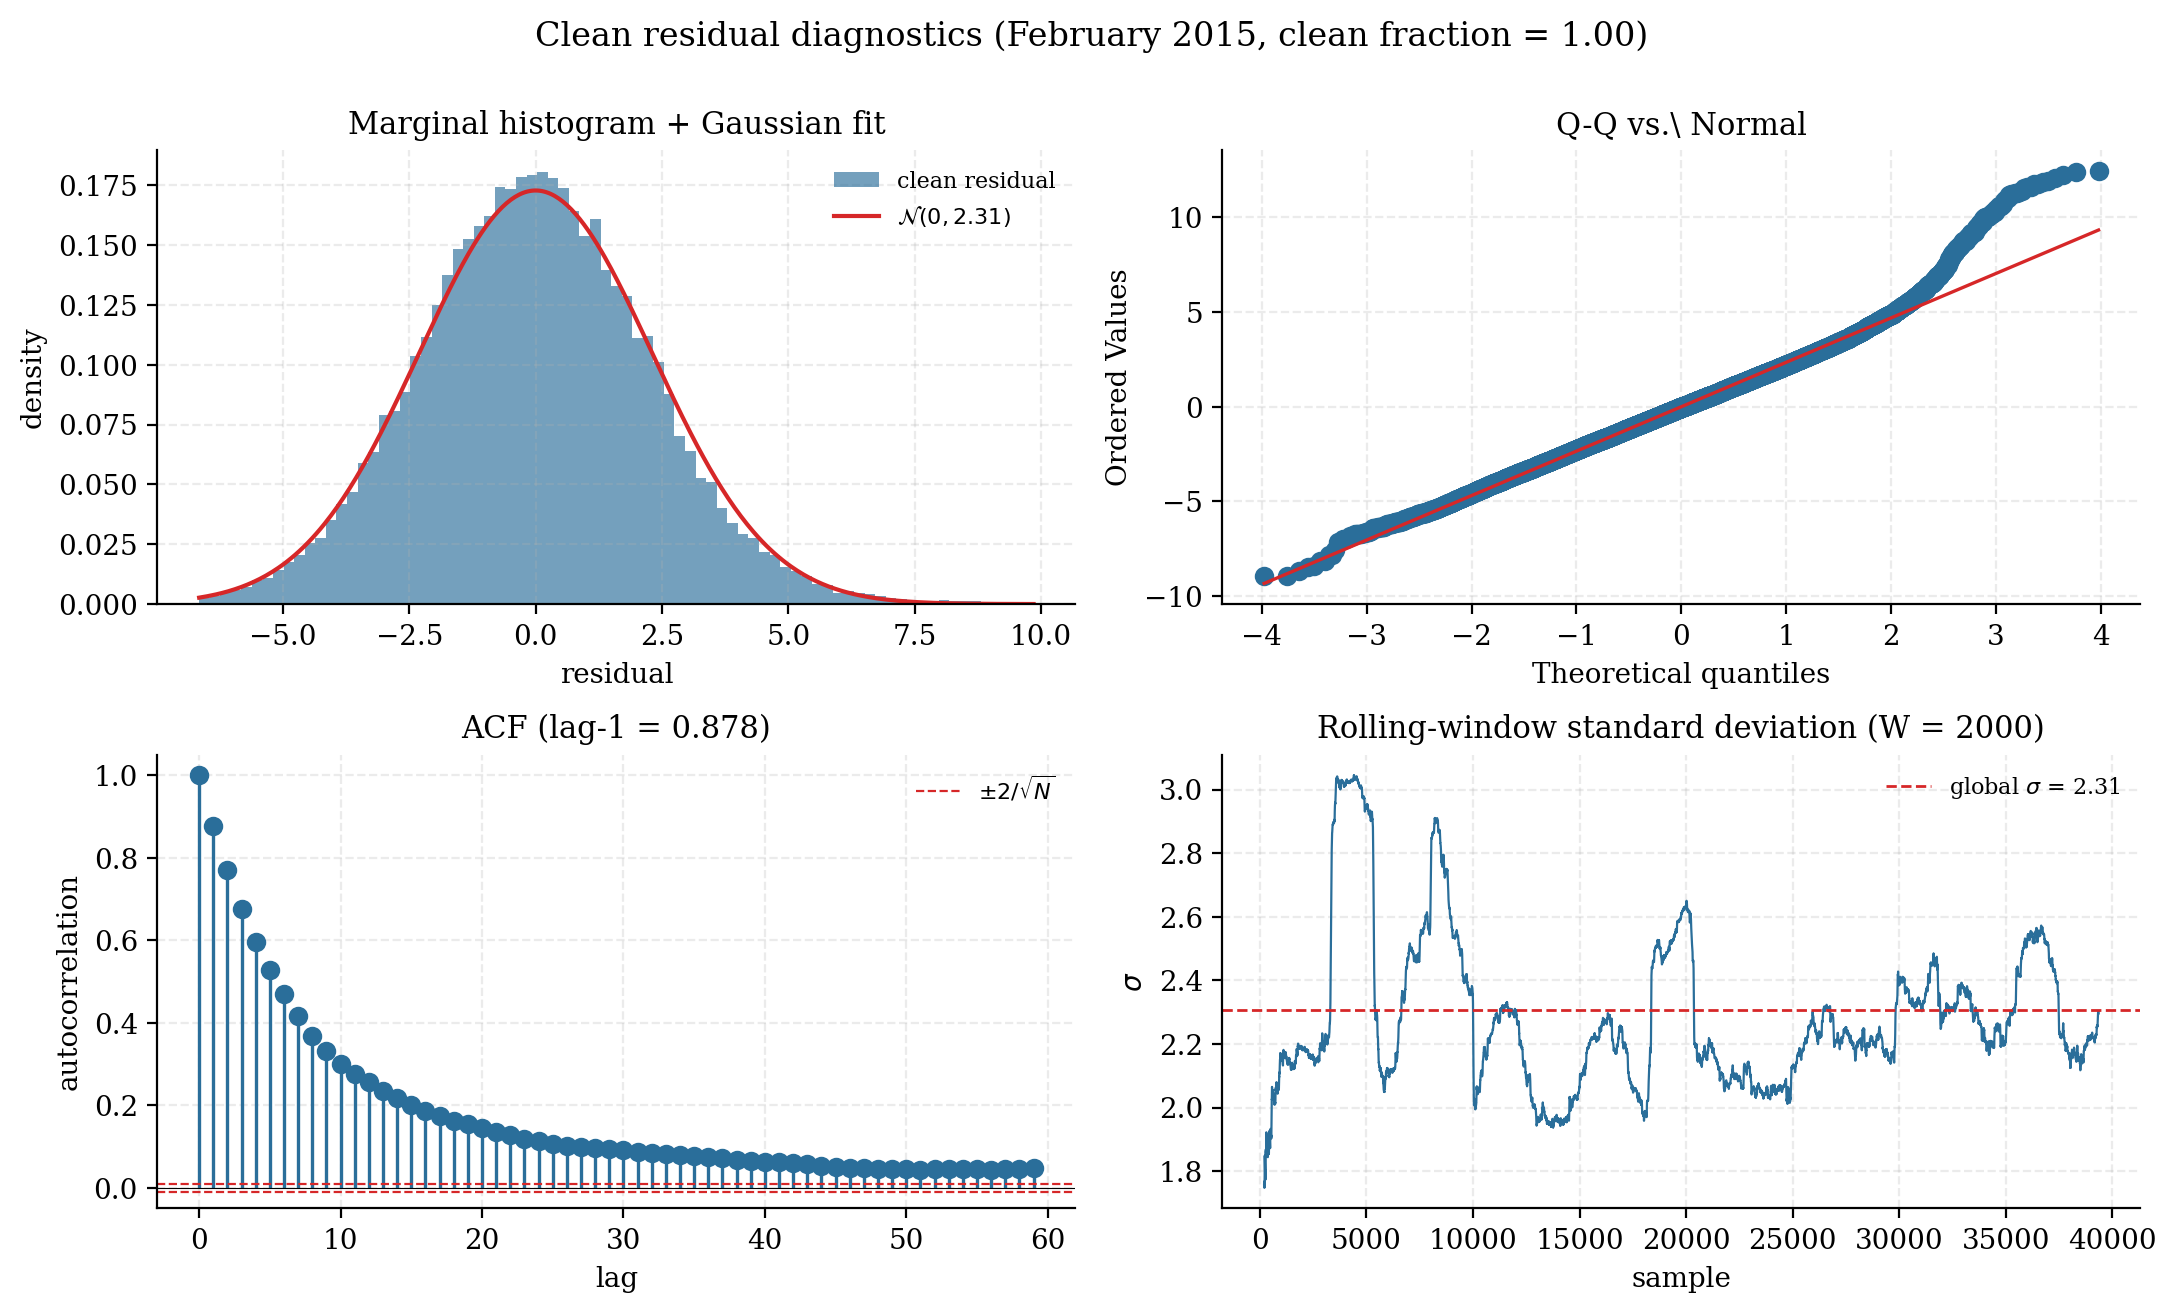
\includegraphics[width=\linewidth]{figures/noise_clean_residual}
    \caption{Diagnostics on the masked residual of February 2015.
    \textbf{Top-left}: marginal histogram, near-perfectly fit by
    $\mathcal{N}(0, 2.21)$. \textbf{Top-right}: Q-Q plot vs.\ Normal,
    on the diagonal. \textbf{Bottom-left}: autocorrelation function on
    the clean segment --- $\mathrm{ACF}(1) = 0.864$, decaying smoothly
    to zero by lag $\sim 30$. \textbf{Bottom-right}: rolling
    standard deviation, stationary around the global value.}
    \label{fig:reanal-clean-residual}
\end{figure}

The marginal histogram and the Q-Q plot are essentially perfect
Gaussian fits: the marginal distribution of the clean residual is, to
a very good approximation, $\mathcal{N}(0, \sigma^2)$. That part of
the v1 noise model \cref{eq:v1-noise-model} is correct.

The autocorrelation panel, however, is not. Under an IID-Gaussian
residual, $\mathrm{ACF}(k)$ should sit inside the $\pm 2 / \sqrt{N}$
band for all $k \geq 1$. The empirical ACF instead starts at $0.864$
at lag $1$ and decays smoothly to zero only around lag $30$. The same
pattern holds in every month
(\cref{tab:reanal-noise}).

\begin{table}[H]
    \centering
    \footnotesize
    \begin{tabular}{lcccccc}
        \toprule
        Month & Clean frac.\ & $\sigma$ & Skew & Exc.\ kurt &
        $\mathrm{ACF}(1)$ & AR(1) $\varphi$ \\
        \midrule
        24/02/2015 & $0.927$ & $2.21$ & $+0.08$ & $+0.10$ & $0.864$ & $0.872$ \\
        30/04/2015 & $0.909$ & $2.34$ & $+0.22$ & $+1.01$ & $0.867$ & $0.867$ \\
        22/06/2015 & $0.953$ & $2.36$ & $+0.60$ & $+3.74$ & $0.850$ & $0.856$ \\
        20/10/2015 & $0.917$ & $2.30$ & $+0.24$ & $+1.07$ & $0.861$ & $0.864$ \\
        \midrule
        \textbf{Average} & $0.927$ & $2.30$ & $+0.29$ & $+1.48$ &
        $\mathbf{0.861}$ & $\mathbf{0.865}$ \\
        \bottomrule
    \end{tabular}
    \caption{Event-masked residual statistics. The lag-1 ACF $\approx
    0.86$ is essentially identical to the fitted AR(1) coefficient
    (which is the MLE for $\varphi$ in a Gaussian AR(1)). The marginal
    standard deviation $\sigma = 2.30$ matches the value reported in
    \cref{tab:real-stats}; what \cref{tab:real-stats} did not see is
    the strong serial correlation behind it.}
    \label{tab:reanal-noise}
\end{table}

The clean residual is well described by a first-order autoregressive
Gaussian process:
\begin{equation}
    r_t = \varphi\, r_{t-1} + \varepsilon_t,
    \quad \varepsilon_t \overset{\text{iid}}{\sim}
        \mathcal{N}(0, \sigma_\varepsilon^2),
    \quad \varphi \approx 0.86,
    \label{eq:ar1-noise}
\end{equation}
with stationary marginal variance
$\sigma_r^2 = \sigma_\varepsilon^2 / (1 - \varphi^2)$. Plugging in
$\sigma_r = 2.30$ and $\varphi = 0.86$ gives an innovation standard
deviation $\sigma_\varepsilon \approx 1.17$.

\section{AR-order selection: is AR(1) enough?}
\label{sec:reanalysis-arorder}

\Cref{eq:ar1-noise} is the simplest model consistent with the
short-lag autocorrelation. We test whether a higher-order AR fits the
data better by fitting AR$(p)$ for $p \in \{1, 2, 3, 5, 10\}$ on the
clean residual of each month and comparing AIC, BIC, and the whiteness
of the AR innovations.

\Cref{fig:reanal-ar1-innov} shows the diagnostics on the AR(1)
innovations.

\begin{figure}[H]
    \centering
    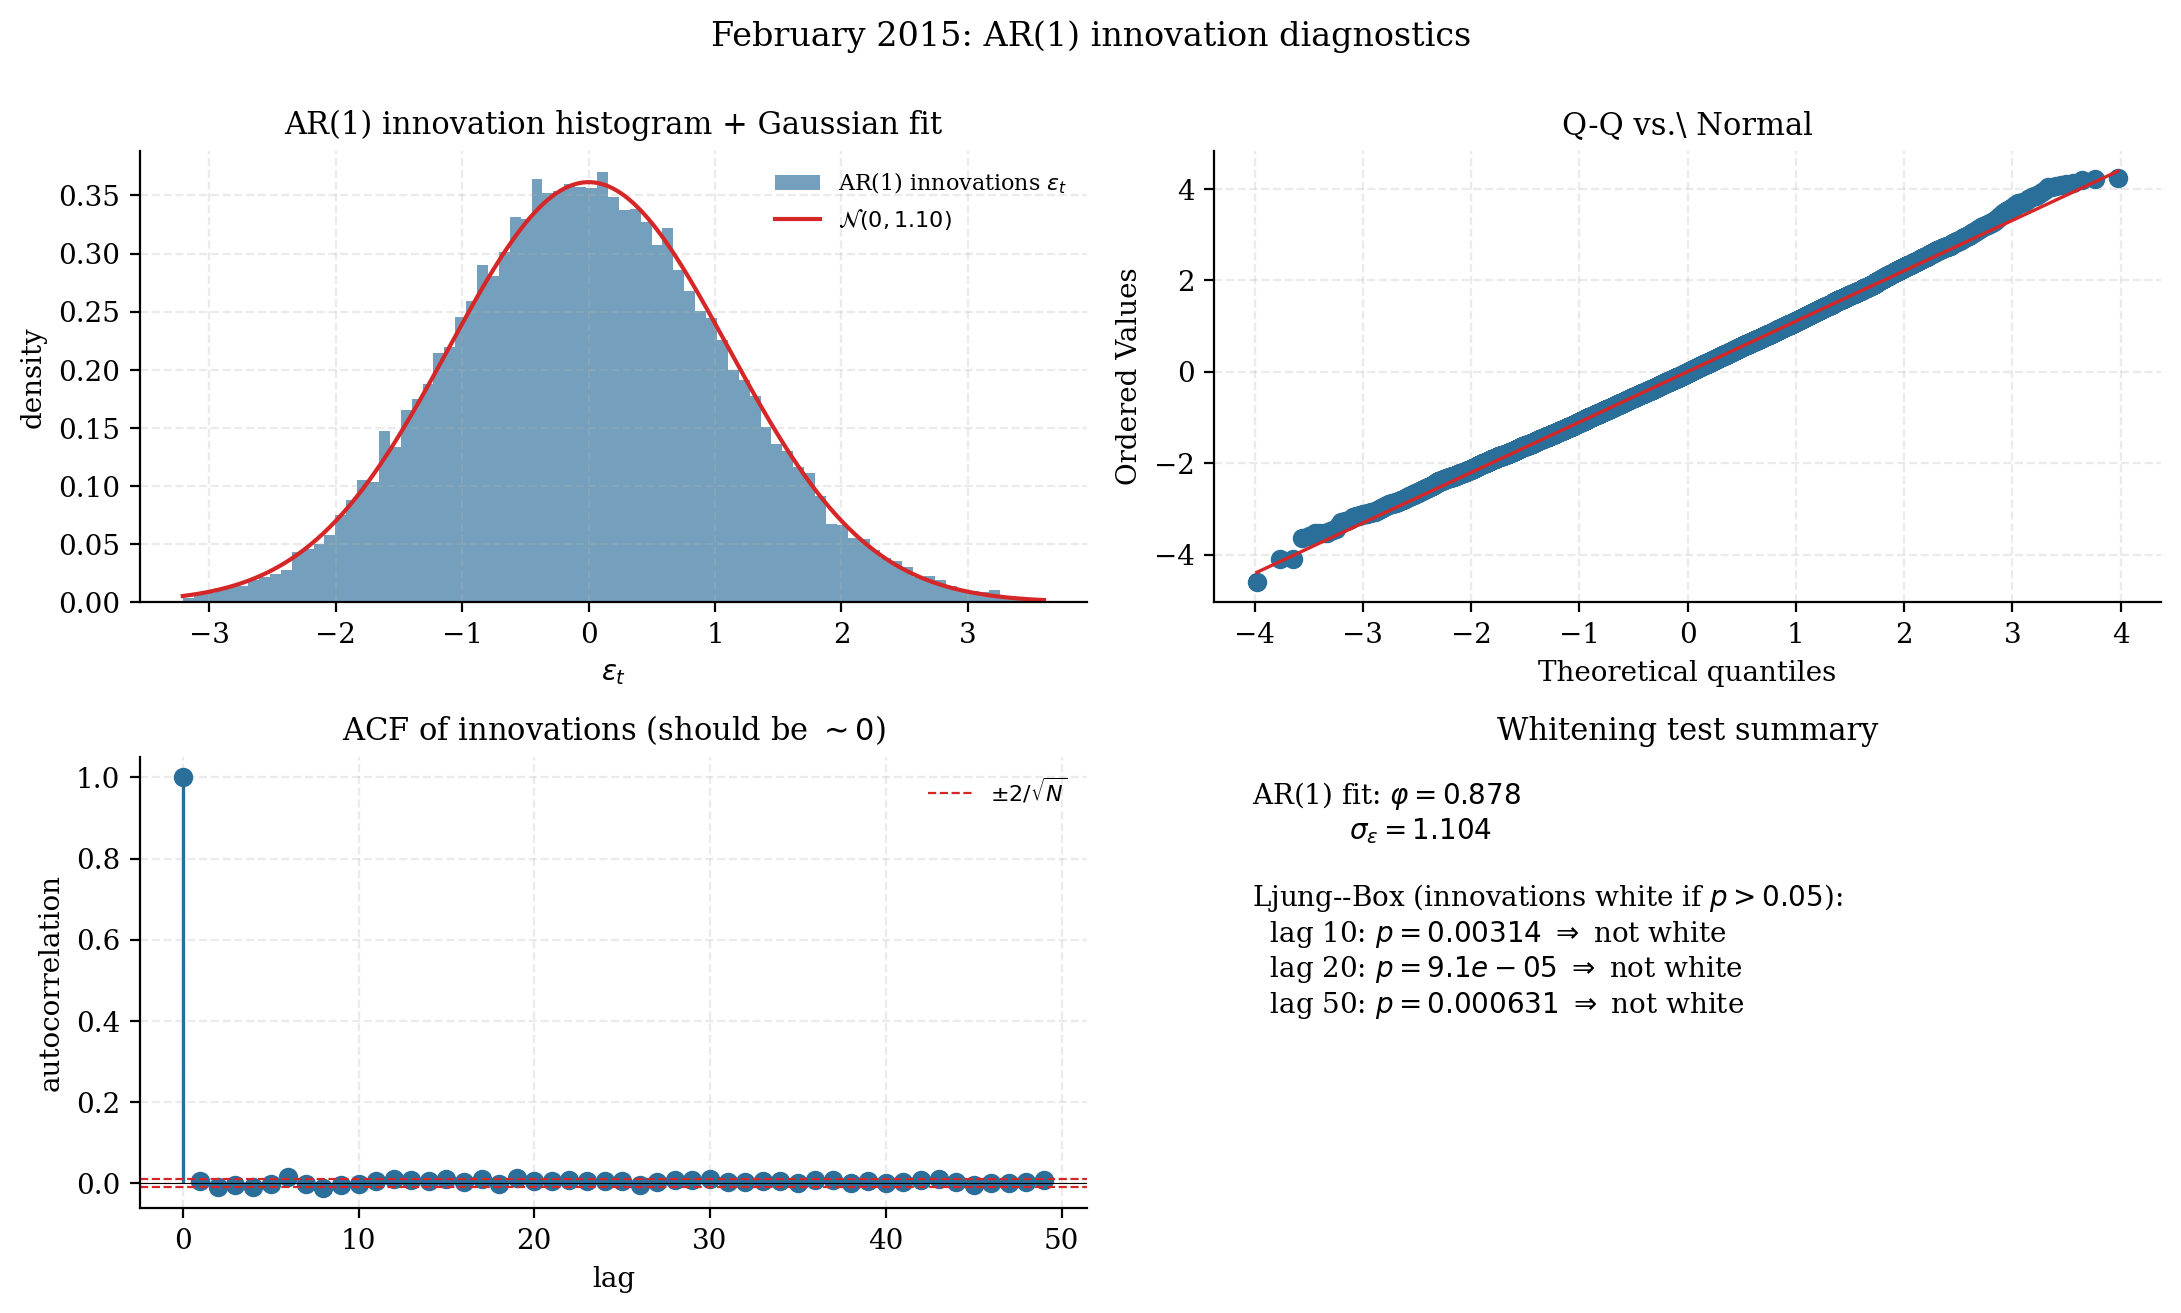
\includegraphics[width=\linewidth]{figures/noise_ar1_innov}
    \caption{AR(1) innovation diagnostics, February 2015. Top-left:
    histogram + Gaussian fit. Top-right: Q-Q vs.\ Normal. Bottom-left:
    ACF of innovations, with bars inside or barely outside the
    $\pm 2 / \sqrt{N}$ band. Bottom-right: Ljung--Box summary.}
    \label{fig:reanal-ar1-innov}
\end{figure}

BIC --- which penalises higher orders more heavily --- selects AR(1)
in three months out of four. Ljung--Box on AR(1) innovations formally
rejects whiteness at the $5\%$ level in three months, with residual
autocorrelations of $|\hat{\rho}_k| \lesssim 0.02$ that are
statistically detectable at $N \approx 38\,000$ but visually
indistinguishable from zero. AR(2) and higher orders are formally
better, but the additional AR coefficients are essentially zero:
$\varphi_2 \approx -0.02$, $\varphi_3 \approx +0.007$, etc.

\begin{figure}[H]
    \centering
    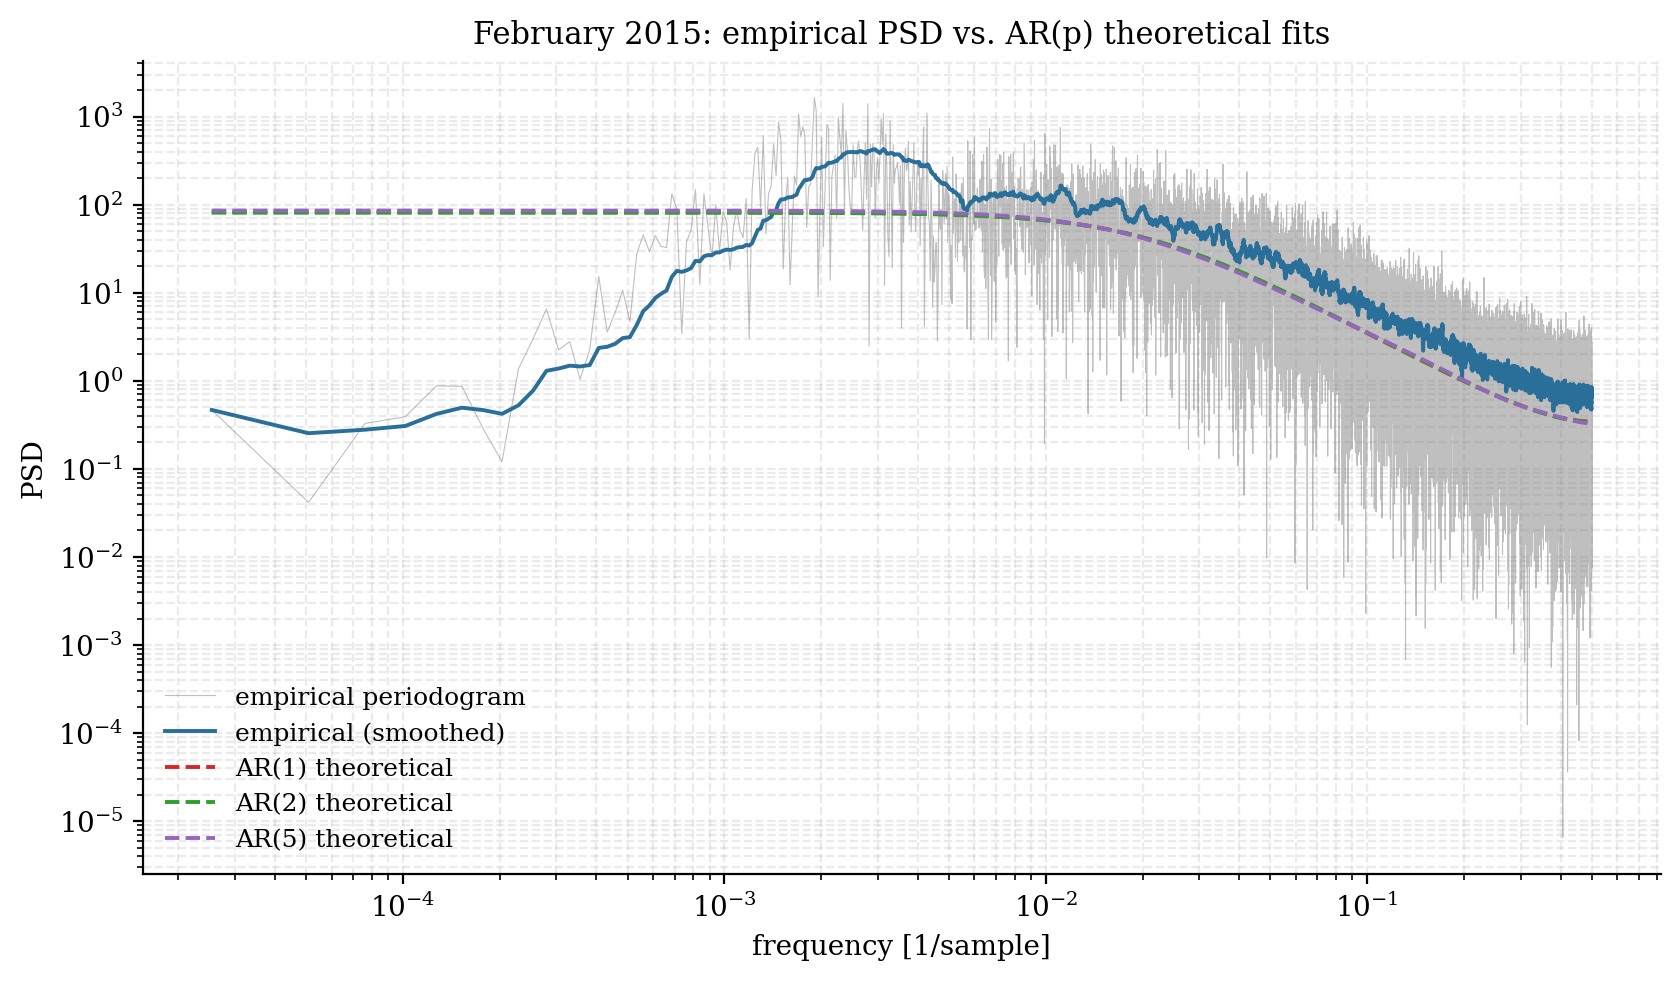
\includegraphics[width=0.85\linewidth]{figures/noise_psd_cmp}
    \caption{Empirical residual periodogram (grey scatter + blue
    smoothed line) against the theoretical PSDs of AR(p) fits. AR(1),
    AR(2) and AR(5) produce essentially indistinguishable theoretical
    spectra, all of which match the empirical periodogram across five
    decades of frequency.}
    \label{fig:reanal-psd-cmp}
\end{figure}

\paragraph{Take-away.} The marginal improvement from increasing the AR
order above $1$ is real but practically negligible at the texture scale
that the convolutional stem cares about. The generator uses
$\varphi = 0.86$, $\sigma_\varepsilon = 1.12$ in \cref{chap:v2gen}.

\subsection{Stationarity}
\label{sec:reanalysis-stability}

Splitting each month into four equal-length chunks and re-fitting
AR(1) on each gives the diagnostics in \cref{fig:reanal-stability}.

\begin{figure}[H]
    \centering
    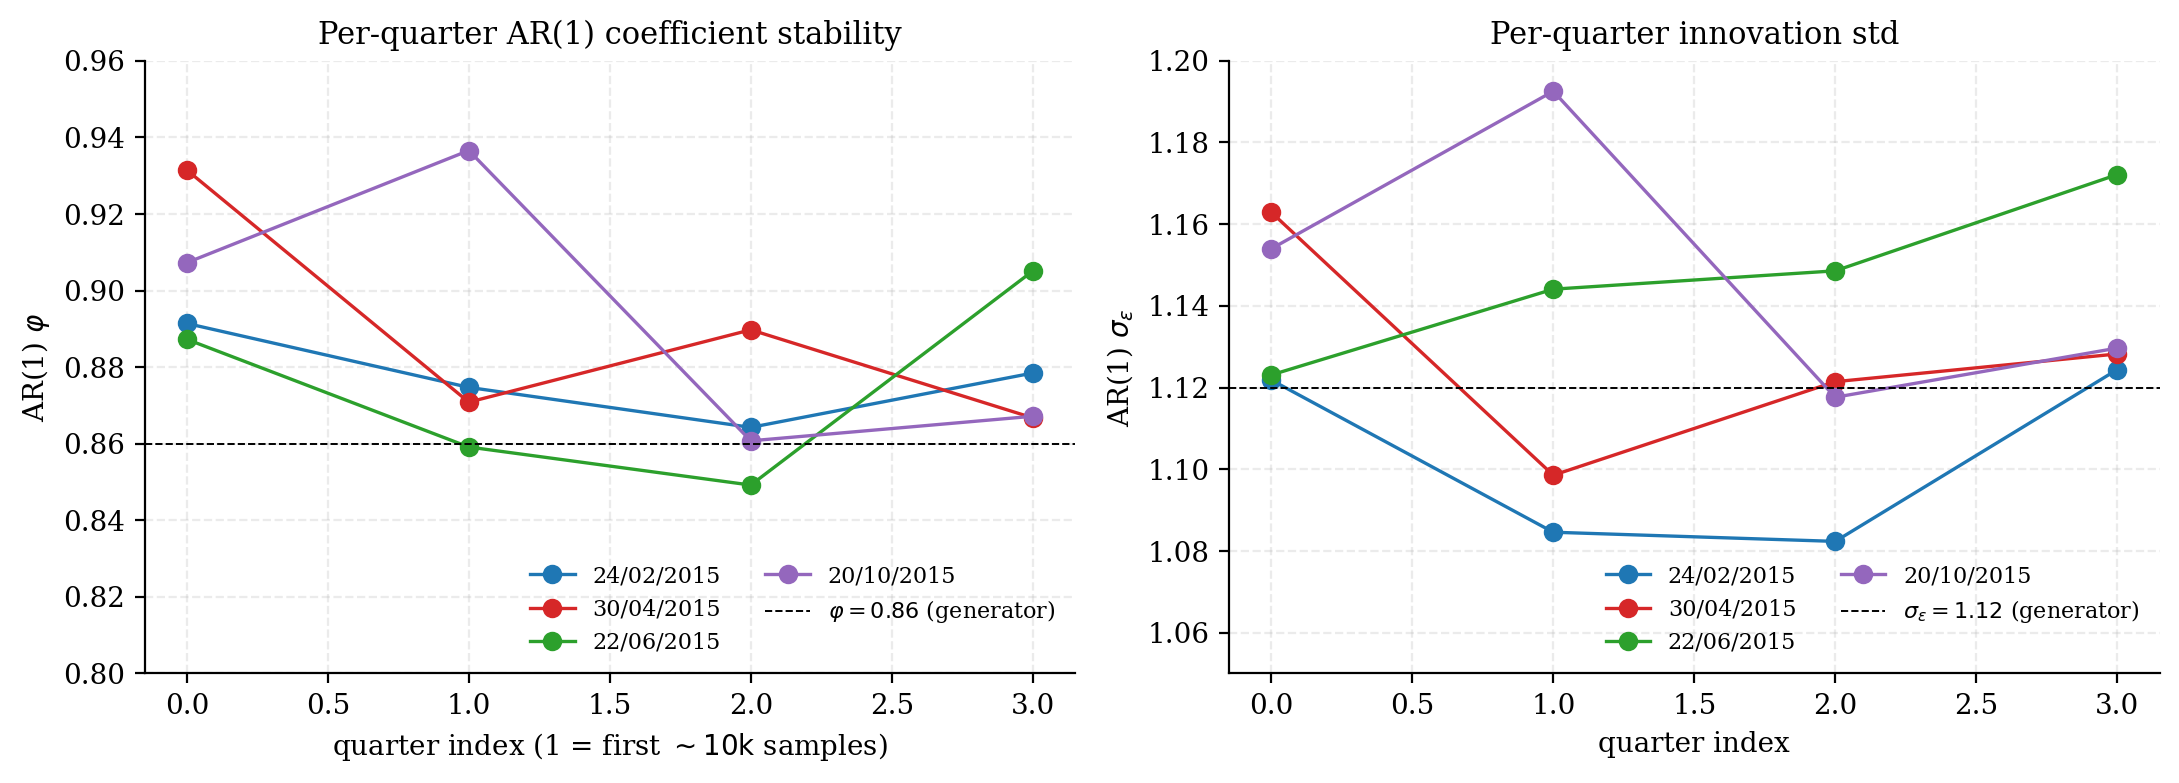
\includegraphics[width=\linewidth]{figures/noise_stability}
    \caption{Per-quarter AR(1) parameter estimates. \textbf{Left}:
    $\varphi$, stable around $\sim 0.87$ except for an early-month
    excursion in October likely caused by a few unmasked outliers.
    \textbf{Right}: innovation std $\sigma_\varepsilon$, stable around
    $\sim 1.12$. The dashed lines mark the values used in the v2
    generator.}
    \label{fig:reanal-stability}
\end{figure}

The estimates are stable to within $\pm 0.04$ for $\varphi$ and
$\pm 0.05$ for $\sigma_\varepsilon$ across the four months. The
generator can safely use a single $(\varphi, \sigma_\varepsilon)$ pair
without sampling them per recording.

\section{Baseline drift: linear, not mean-reverting}
\label{sec:reanalysis-drift}

The Ornstein--Uhlenbeck baseline of \cref{eq:v1-noise-model} is a
\emph{stationary} mean-reverting random walk. A linear fit to the
wide-scale baseline (MA-17280) of each month is reported in
\cref{tab:reanal-drift}.

\begin{table}[H]
    \centering
    \footnotesize
    \begin{tabular}{lccc}
        \toprule
        Month & Linear slope / sample & Total drift over $\sim 40$k samples
              & ADF $p$-value \\
        \midrule
        24/02/2015 & $+7.5 \cdot 10^{-5}$ & $+2.95$ & $0.998$ \\
        30/04/2015 & $+2.1 \cdot 10^{-5}$ & $+0.84$ & $0.944$ \\
        22/06/2015 & $+9.8 \cdot 10^{-5}$ & $+3.87$ & $0.078$ \\
        20/10/2015 & $-1.0 \cdot 10^{-4}$ & $-3.99$ & $0.938$ \\
        \bottomrule
    \end{tabular}
    \caption{Wide-scale baseline drift per month. ADF tests the null
    of a unit root (non-stationary baseline); the null is \emph{not}
    rejected in three months out of four, consistent with seasonal or
    meteorological trends rather than a mean-reverting OU process.}
    \label{tab:reanal-drift}
\end{table}

The slopes are of order $10^{-4}$ counts per sample and their sign
varies across months. An OU process simulating a month-long path with
the v1 parameters returns close to its starting point with high
probability; the real baseline does not. The v2 generator re-tunes the
OU parameters $(\theta, \sigma_{\mathrm{OU}})$ to produce drifts of the
right magnitude over $40$k samples (\cref{sec:v2-changes}).

\section{Hand labels: seventeen plausible events}
\label{sec:reanalysis-labels}

The second prong of the re-analysis is direct hand-labelling of the
real recordings. The helper script \texttt{data-gen/labeling\_view.py}
produces, for each month, several diagnostic views at multiple
smoothing scales (window sizes $15$, $30$, $60$, $120$, $240$ samples)
both on the raw and on a detrended signal, plus per-event zoom-ins.
\Cref{fig:hand-labels-overview} shows the resulting labels on the four
months.

\begin{figure}[H]
    \centering
    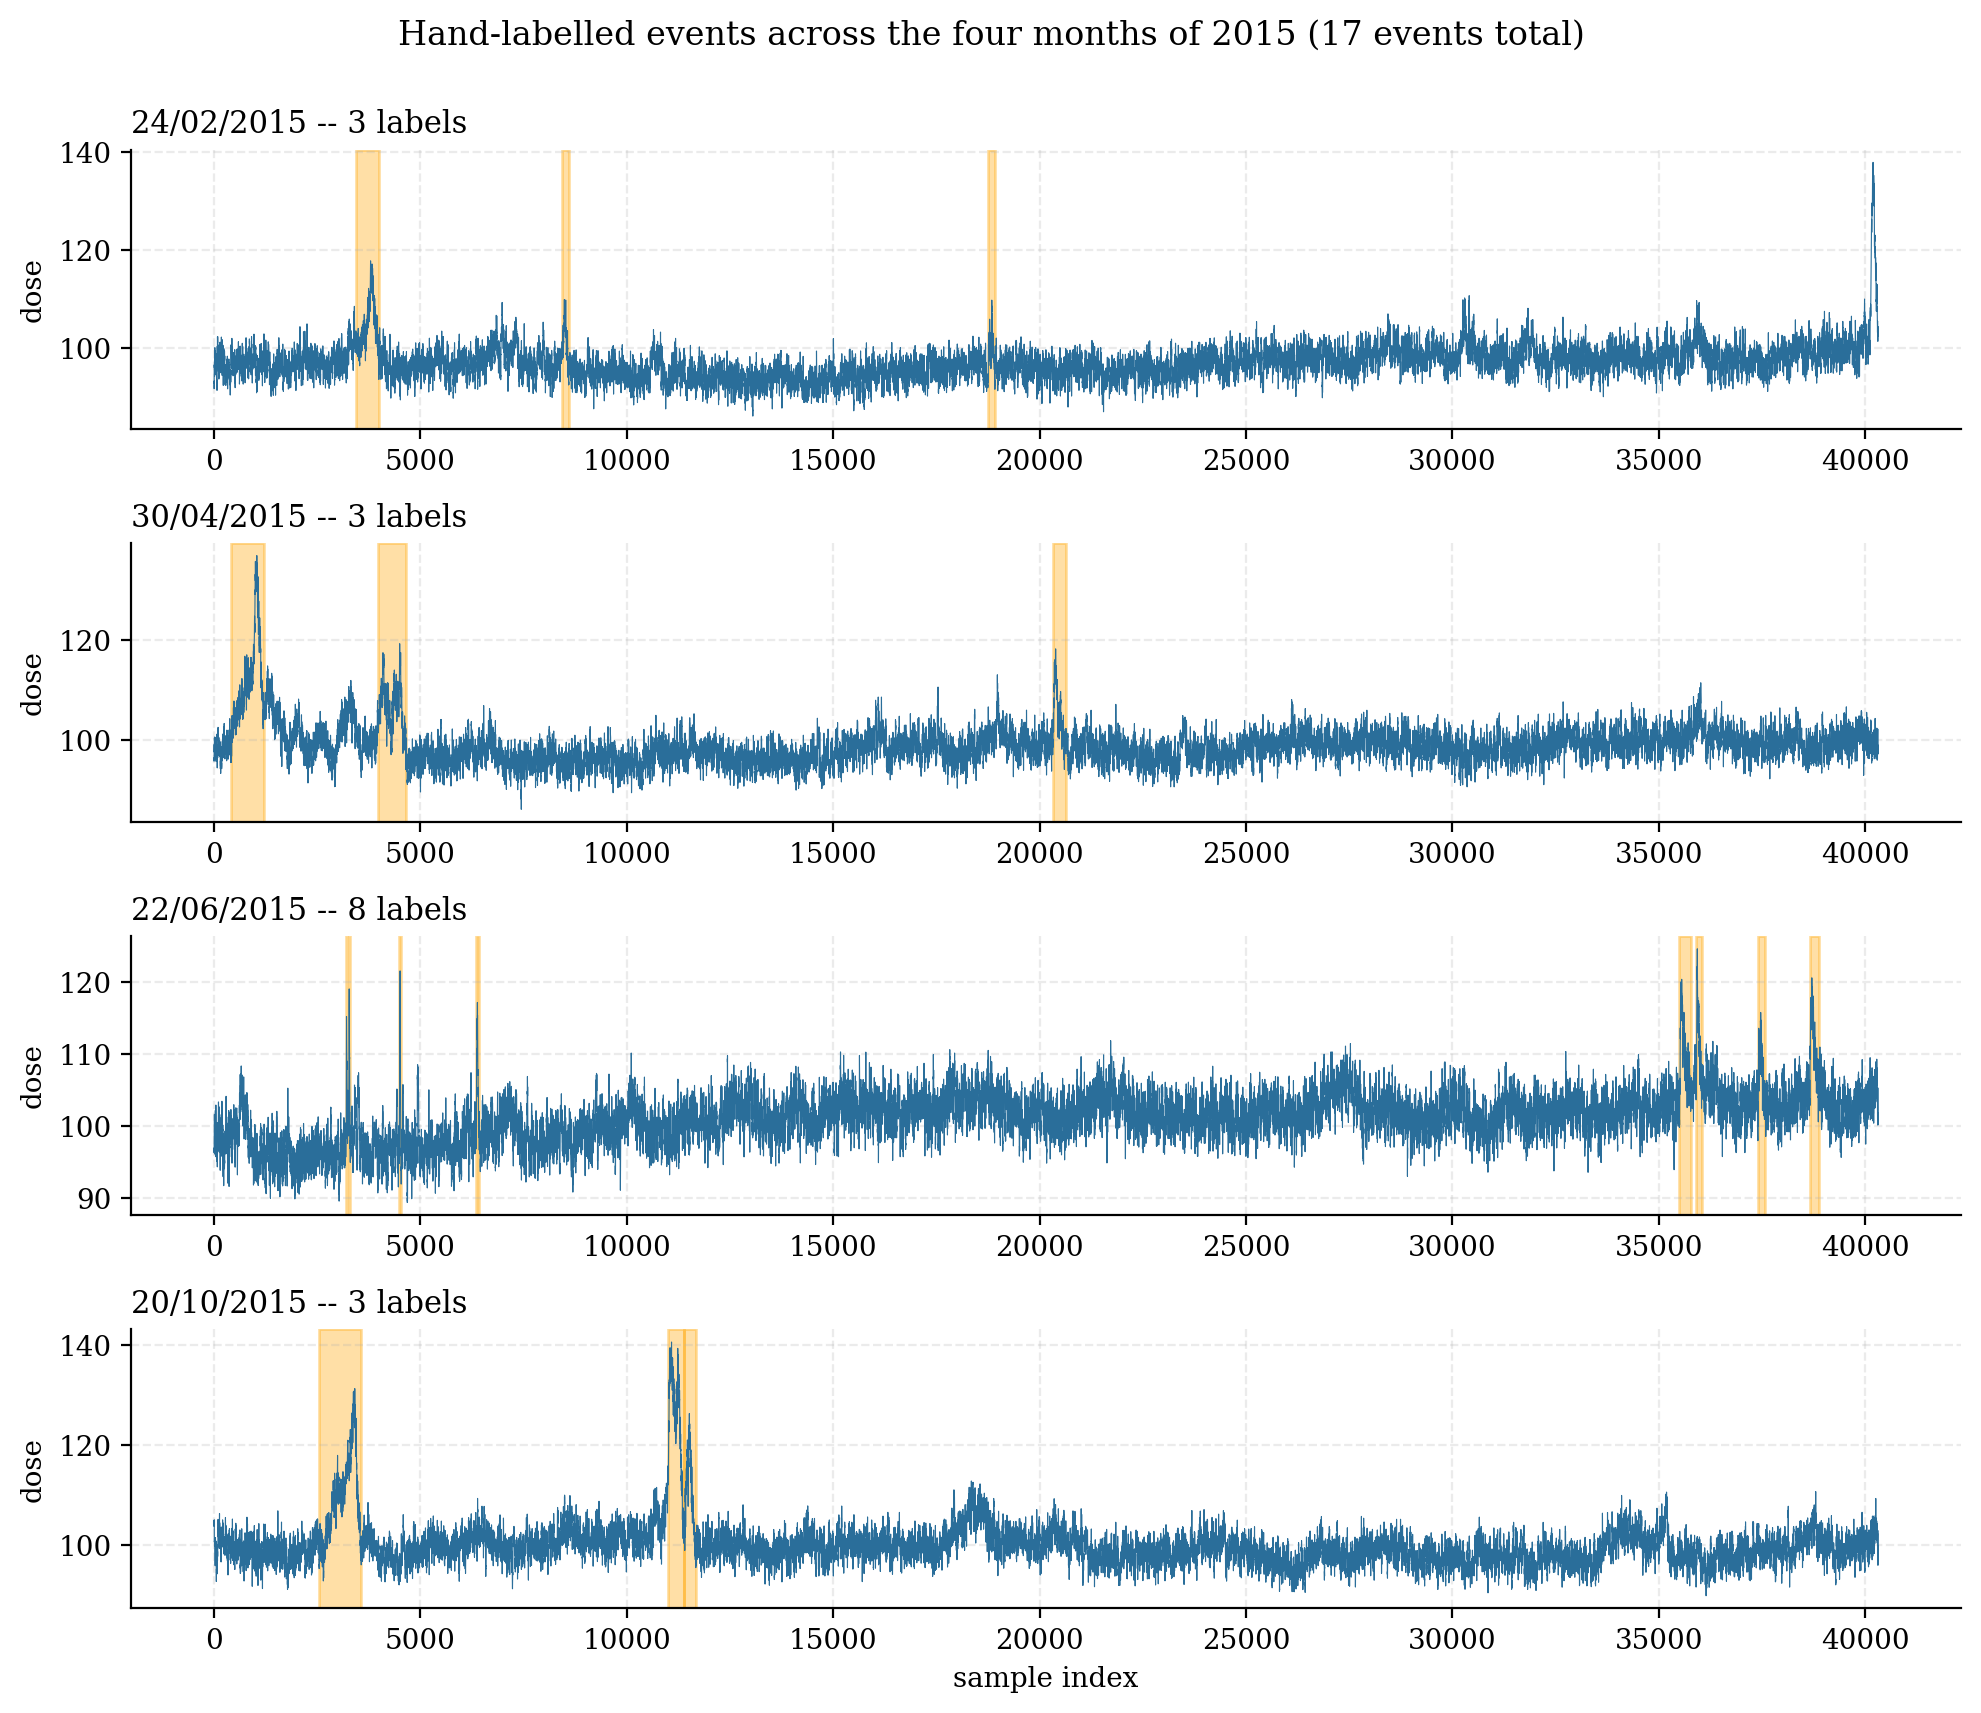
\includegraphics[width=\linewidth]{figures/hand_labels_overview}
    \caption{The four months of real 2015 data with hand-labelled
    event spans (orange). Across the four months there are
    $3 + 3 + 8 + 3 = 17$ labelled events.}
    \label{fig:hand-labels-overview}
\end{figure}

\Cref{fig:hand-labels-zoom} provides a zoomed view of the eight
labelled events in June 2015 --- the most varied month --- with two
smoothing scales overlaid.

\begin{figure}[H]
    \centering
    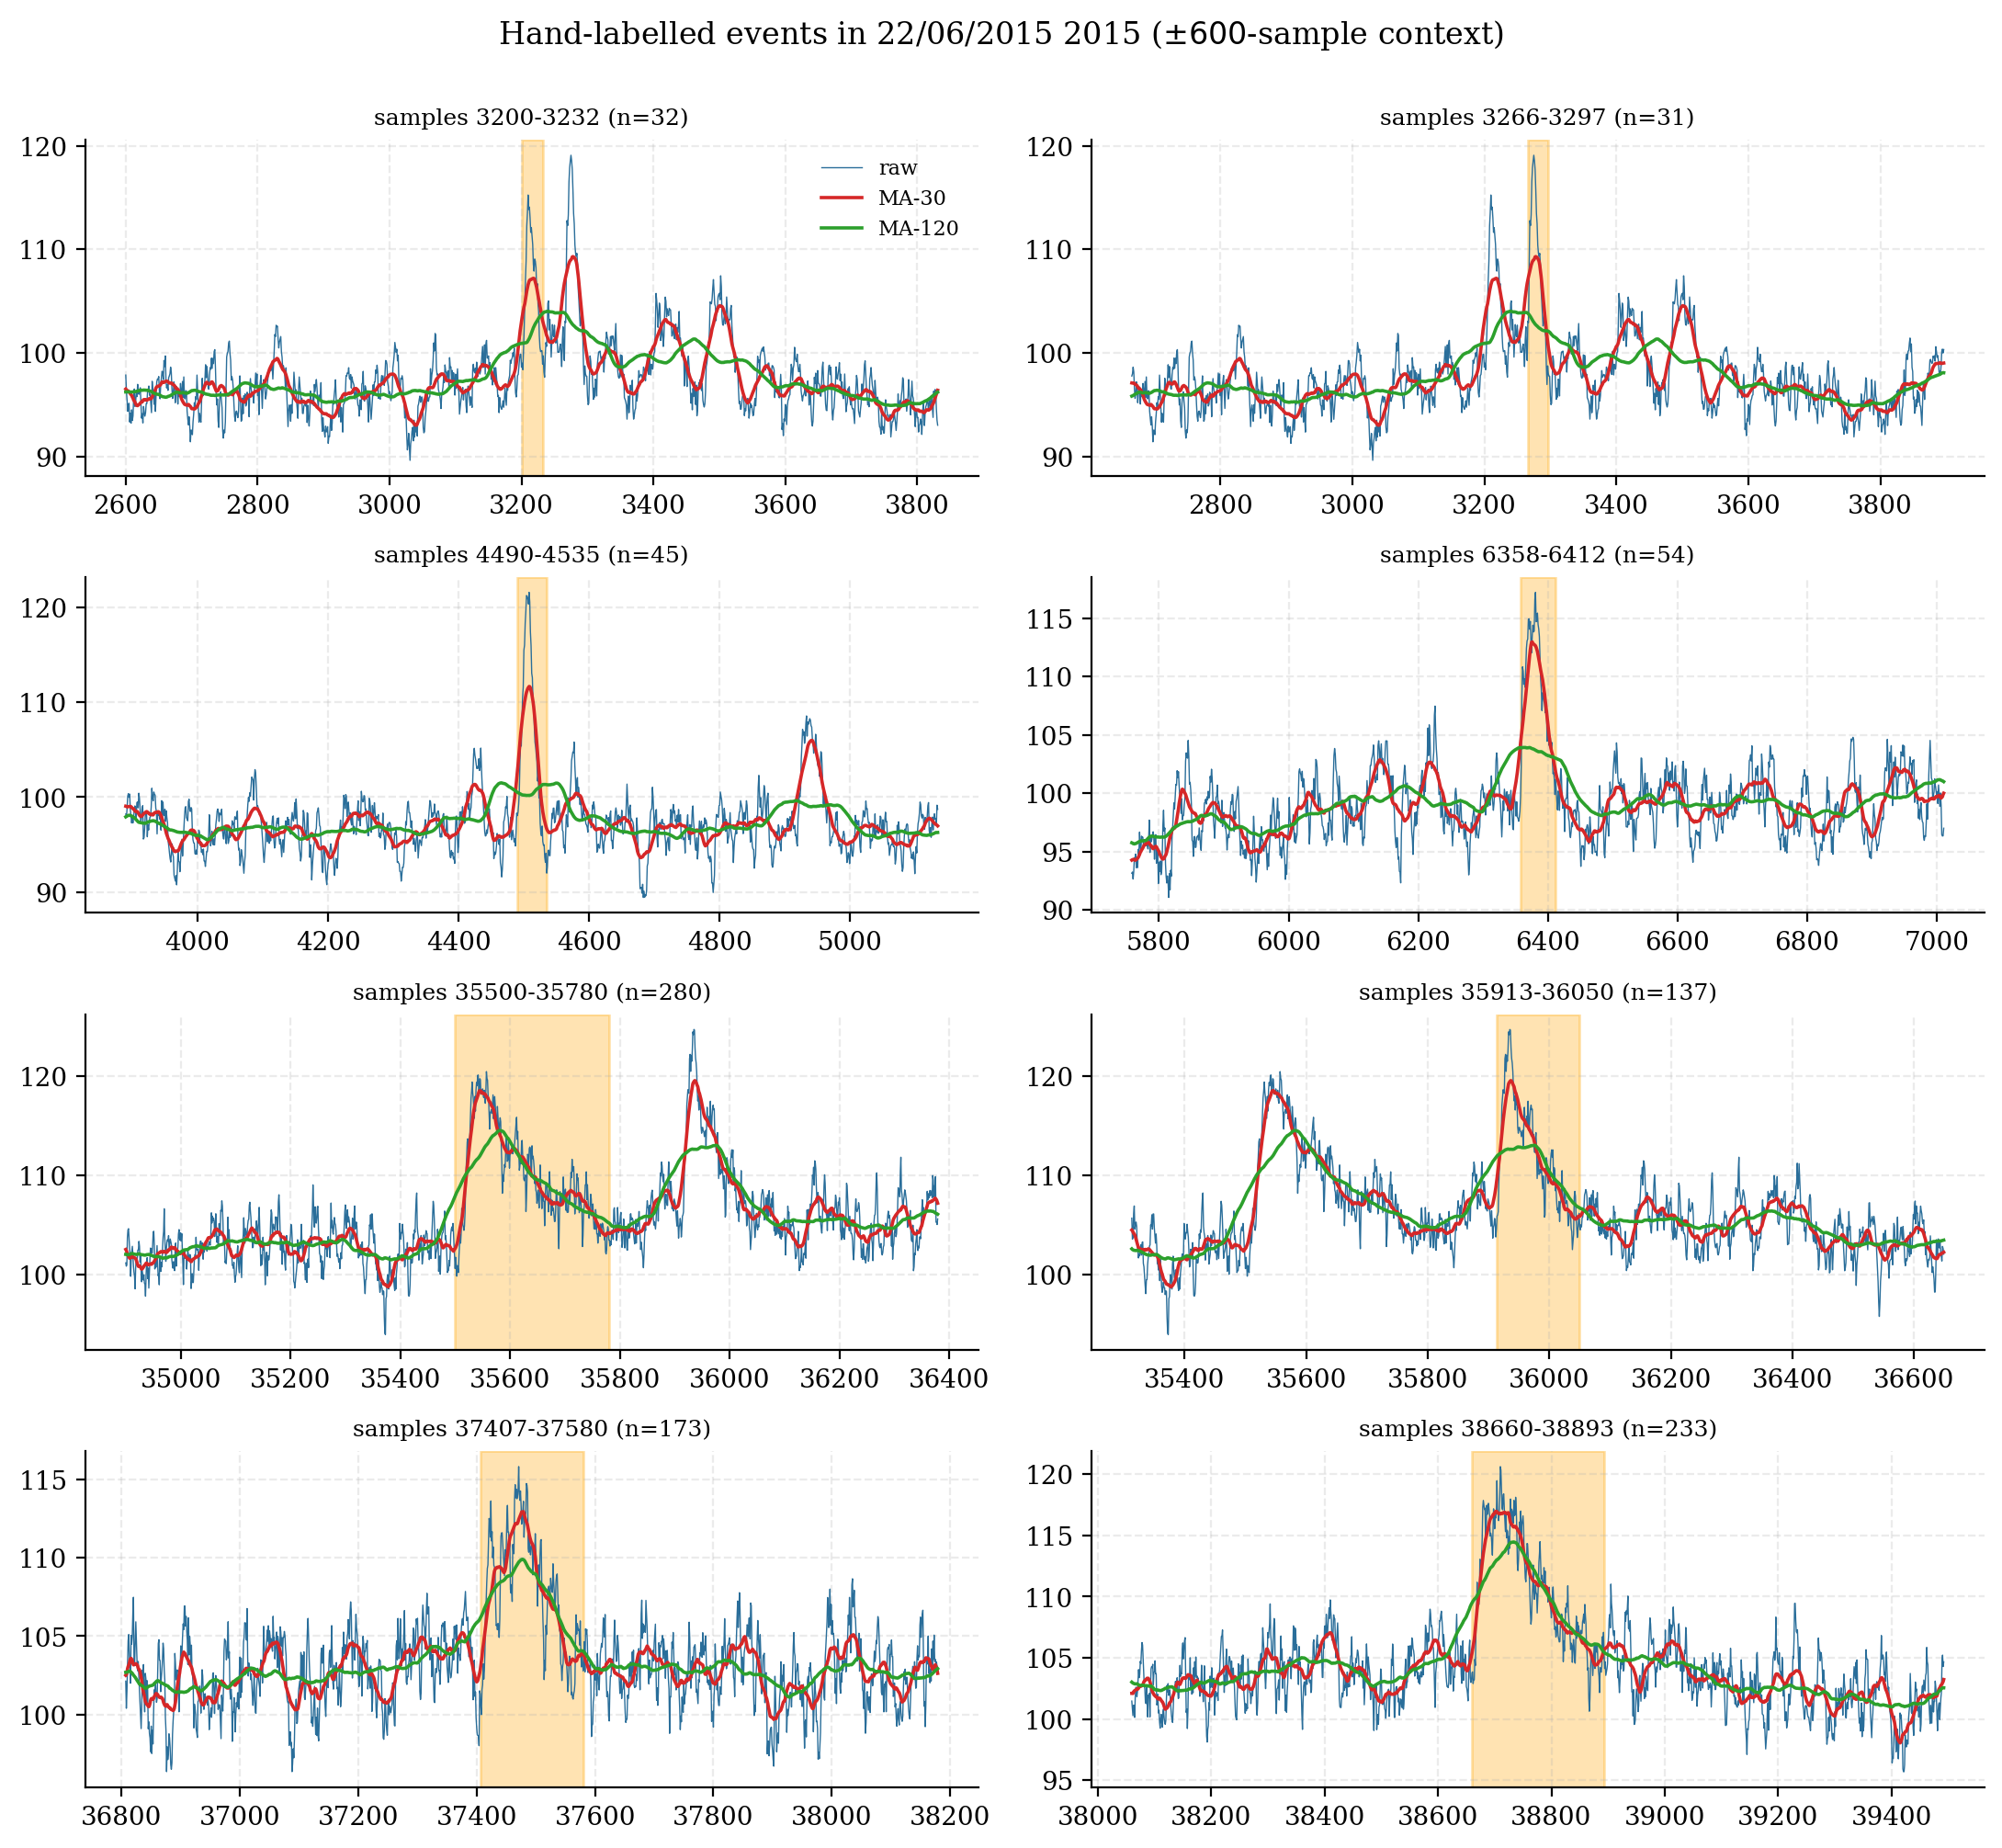
\includegraphics[width=\linewidth]{figures/hand_labels_zoom}
    \caption{Zoomed view around each of the eight hand-labelled events
    in June 2015 ($\pm 600$ samples of context). The orange band marks
    the labelled interval; coloured lines are MA-30 (red) and MA-120
    (green) smoothings. The first four events are very short
    ($30$--$55$ samples) sharp spikes; the last four are longer
    ($138$--$281$ samples), with a mix of bell and asymmetric shapes.}
    \label{fig:hand-labels-zoom}
\end{figure}

\paragraph{Limitations.} The labels are \emph{provisional}, produced
by visual inspection without radiological expertise. Event boundaries
are partly subjective (especially the long decay tail of asymmetric
events) and faint excursions below the rolling $\pm 2\sigma$ band are
not flagged. Both points argue that the most impactful next step
beyond v2 is expert labelling rather than further generator tuning.

\subsection{Empirical event distributions}

Two histograms summarise the empirical labels and constrain the v2
generator (\cref{fig:hand-label-stats}).

\begin{figure}[H]
    \centering
    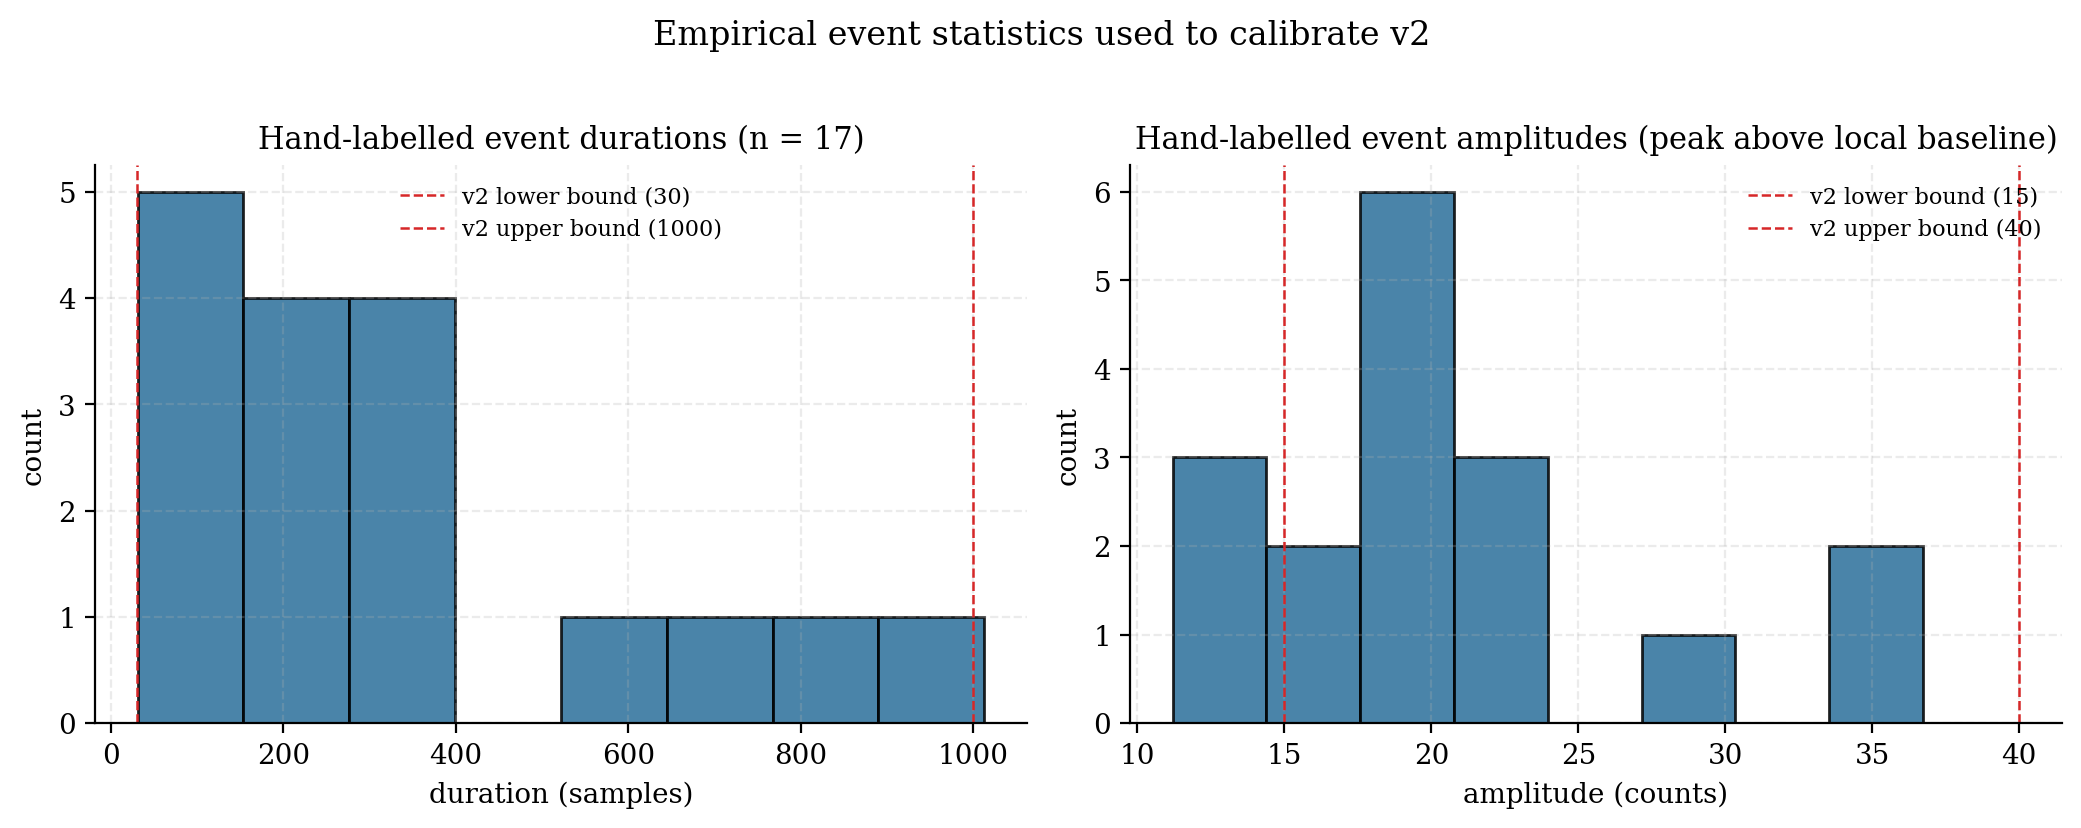
\includegraphics[width=\linewidth]{figures/hand_label_stats}
    \caption{Empirical event statistics from the seventeen hand labels.
    \textbf{Left}: durations span $[32, 1014]$ samples, with most
    events below $400$. \textbf{Right}: peak amplitudes (above the
    MA-4320 local baseline) span $[11.2, 36.8]$ counts. The red dashed
    lines mark the v2 generator's $[30, 1000]$-sample and $[15, 40]$
    count bounds.}
    \label{fig:hand-label-stats}
\end{figure}

\subsection{Shape assignment}

Each labelled event is assigned to its closest template by inspecting
the position of its peak inside the event's interval:
\begin{itemize}[leftmargin=*, itemsep=0.2em]
    \item peak in the central third $\rightarrow$ \texttt{bell}
    ($\sim 53\%$, 9/17 events);
    \item peak in the first third $\rightarrow$ \texttt{fast\_descend}
    ($\sim 18\%$, 3/17 events);
    \item peak in the last third $\rightarrow$ \texttt{fast\_ascend}
    ($\sim 29\%$, 5/17 events).
\end{itemize}
None of the labelled events has the multi-peak structure of \texttt{M},
the plateau-with-bumps profile of \texttt{bell\_sq}, or the sustained
square profile of \texttt{square}. The three v1 templates with no
empirical counterpart are dropped in v2.

\subsection{Polarity}

All $17$ events are positive excursions above the local baseline. No
labelled event is a downward dip. The v1 generator already produced
only positive anomalies; v2 keeps that as a deliberate choice rather
than a coincidence.

\section{Targets for the v2 generator}
\label{sec:reanalysis-targets}

Putting \cref{sec:reanalysis-noise,sec:reanalysis-arorder,%
sec:reanalysis-drift,sec:reanalysis-labels} together, the v2 generator
needs to reproduce:

\begin{enumerate}[leftmargin=*, itemsep=0.2em]
    \item \textbf{AR(1) Gaussian high-frequency noise}, with
    $\varphi = 0.86$ and $\sigma_\varepsilon = 1.12$ (marginal std
    $\sigma_r = 2.30$).
    \item \textbf{Baseline drift on the order of $\pm 3$--$4$ counts}
    over a $40$k-sample recording.
    \item \textbf{Anomaly amplitudes in $[15, 40]$ counts}
    (log-uniform), \emph{absolute} (no longer multiples of $\sigma$).
    \item \textbf{Anomaly durations in $[30, 1000]$ samples}
    (log-uniform).
    \item \textbf{Anomaly density $\sim 1.5$ events per $10\text{k}$
    samples} (slightly above the empirical $1.05$ to give the
    classifier a few extra training examples).
    \item \textbf{Three templates only}: \texttt{bell},
    \texttt{fast\_ascend}, \texttt{fast\_descend}.
\end{enumerate}

The acceptance test runs
\texttt{data-gen/analyze\_noise\_model.py} on a chunk of the v2 output
and checks that the AR(1) parameters, the marginal residual statistics,
and the Ljung--Box innovation whiteness all sit within sampling noise
of the targets above. The next chapter describes the v2 generator that
meets the acceptance test.
